\documentclass[aspectratio=169,11pt]{beamer}

% Shared style (ib-tutorials.sty at the repo root).
\makeatletter\def\input@path{{./}{../}}\makeatother
\usepackage{ib-tutorials}

\usepackage[utf8]{inputenc}
\usepackage{amsmath,amssymb}
\usepackage{booktabs}
\usepackage{array}
\usepackage{graphicx}
\usepackage{xcolor}
\usepackage{listings}
\usepackage{tikz}
\usetikzlibrary{arrows.meta,positioning,shapes.geometric,fit,calc}
\usepackage{hyperref}

\graphicspath{{pictures/1-getting-set-up/}{../pictures/1-getting-set-up/}}
\newcommand{\sourcecredit}[1]{\vfill\hfill{\tiny\textcolor{DarkGray}{#1}}}
\newcolumntype{L}[1]{>{\raggedright\arraybackslash}p{#1}}

\lstset{
  basicstyle=\ttfamily\scriptsize\color{BlackGray},
  keywordstyle=\color{NavyBlue}\bfseries,
  commentstyle=\color{DarkGray}\itshape,
  stringstyle=\color{OliveGreen},
  showstringspaces=false,
  columns=fullflexible,
  keepspaces=true,
  frame=single,
  framerule=0.4pt,
  rulecolor=\color{LightGray},
  backgroundcolor=\color{LightGray!30},
  xleftmargin=0.25em,
  xrightmargin=0.25em,
  breaklines=true,
  breakatwhitespace=true
}
\lstdefinestyle{shell}{morecomment=[l]{\#}}
\lstdefinestyle{tiny}{basicstyle=\ttfamily\tiny\color{BlackGray}}
\lstdefinestyle{slurm}{}

\title[Computing environment]{Computing on Puma, the UA cluster}
\subtitle{Accounts, logging in, files, the shell, and Slurm}
\author[Miller]{Laura A. Miller}
\institute[UArizona]{Department of Mathematics, University of Arizona}
\date{Using IB Software \textbullet\ Part I \textbullet\ Chapter 1}

\tikzset{
  box/.style={draw=DarkGray,rounded corners=1pt,fill=LightGray!45,align=center,inner sep=3pt,font=\scriptsize},
  hot/.style={draw=RubineRed,thick,rounded corners=1pt,fill=RubineRed!8,align=center,inner sep=3pt,font=\scriptsize},
  arr/.style={-{Stealth[length=2mm]},DarkGray},
  lab/.style={font=\tiny,text=DarkGray}
}

\begin{document}

% 1
\begin{frame}[plain]
\maketutorialtitlepanel{%
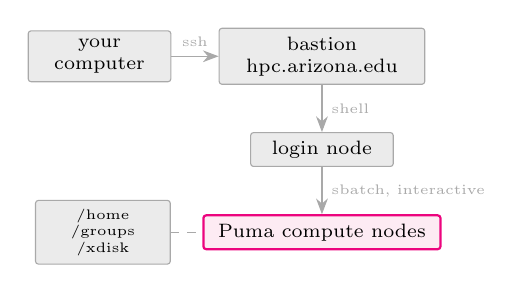
\begin{tikzpicture}[node distance=4mm]
  \node[box,text width=16mm] (me) {your\\computer};
  \node[box,right=6mm of me,text width=24mm] (bast) {bastion\\\code{hpc.arizona.edu}};
  \node[box,below=6mm of bast,text width=16mm] (login) {login node};
  \node[hot,below=6mm of login,text width=28mm] (comp) {Puma compute nodes};
  \draw[arr] (me) -- node[lab,above]{ssh} (bast);
  \draw[arr] (bast) -- node[lab,right]{\code{shell}} (login);
  \draw[arr] (login) -- node[lab,right]{\code{sbatch}, \code{interactive}} (comp);
  \node[box,left=4mm of comp,text width=15mm,font=\tiny] (st) {\code{/home} \code{/groups}\\\code{/xdisk}};
  \draw[DarkGray,dashed] (st) -- (comp);
\end{tikzpicture}}
\end{frame}

% 2
\begin{frame}{Learning goals}
By the end of this chapter you should be able to:
\begin{enumerate}
  \item get an HPC account and join your PI's group;
  \item log in to Puma by SSH or through Open OnDemand;
  \item move files between your computer and the cluster;
  \item choose where to keep code, simulations and results;
  \item work in the Linux shell: navigate, edit files, and write short scripts;
  \item run work on compute nodes, interactively or as Slurm batch jobs, and check what a job used.
\end{enumerate}
\vspace{3mm}
\begin{punchbox}
\small Since August 2026 Puma is the University of Arizona's only HPC cluster: El Gato was shut down on 29 July 2026 and Ocelote on 17 August 2026. Older course notes for Ocelote, El Gato, and UNC's Kure, KillDevil, Dogwood and Longleaf clusters are kept in Part X, chapter X1.
\end{punchbox}
\end{frame}

% 3
\begin{frame}{How the cluster is organized}
\begin{columns}[c,onlytextwidth]
\begin{column}{0.48\textwidth}
\centering
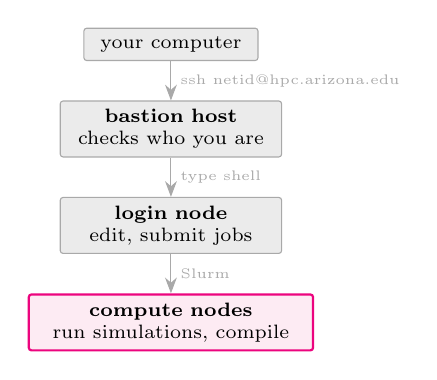
\begin{tikzpicture}[node distance=5mm]
  \node[box,text width=20mm] (me) {your computer};
  \node[box,below=of me,text width=26mm] (bast) {\textbf{bastion host}\\checks who you are};
  \node[box,below=of bast,text width=26mm] (login) {\textbf{login node}\\edit, submit jobs};
  \node[hot,below=of login,text width=34mm] (comp) {\textbf{compute nodes}\\run simulations, compile};
  \draw[arr] (me) -- node[lab,right]{\code{ssh netid@hpc.arizona.edu}} (bast);
  \draw[arr] (bast) -- node[lab,right]{type \code{shell}} (login);
  \draw[arr] (login) -- node[lab,right]{Slurm} (comp);
\end{tikzpicture}
\end{column}
\begin{column}{0.49\textwidth}
\begin{itemize}\small
  \item The \textbf{bastion host} only checks your NetID, password and Duo. It stores no files and has no software.
  \item A \textbf{login node} is shared by everyone who is logged in. Edit files and submit jobs there.
  \item \textbf{Compute nodes} do the work. You reach them through \textbf{Slurm}, the scheduler, which starts your job when the cores you asked for are free.
  \item \alr{Never run simulations or builds on a login node.} Software modules are not even available there.
\end{itemize}
\end{column}
\end{columns}
\end{frame}

% 4
\begin{frame}{Getting an HPC account}
\begin{columns}[T,onlytextwidth]
\begin{column}{0.48\textwidth}
\begin{enumerate}\small
  \item Create your account at \url{https://portal.hpc.arizona.edu} with your NetID.
  \item If you are not faculty, ask a faculty member, your PI, to sponsor you: enter their email address on the portal's sponsorship page.
  \item Your PI approves you and adds you to their \textbf{group}. The group name (for example \code{lauram9}) is what you put after \code{--account} in job scripts.
\end{enumerate}
\small Your sponsor needs their own HPC account before they can sponsor anyone.
\end{column}
\begin{column}{0.49\textwidth}
\centering
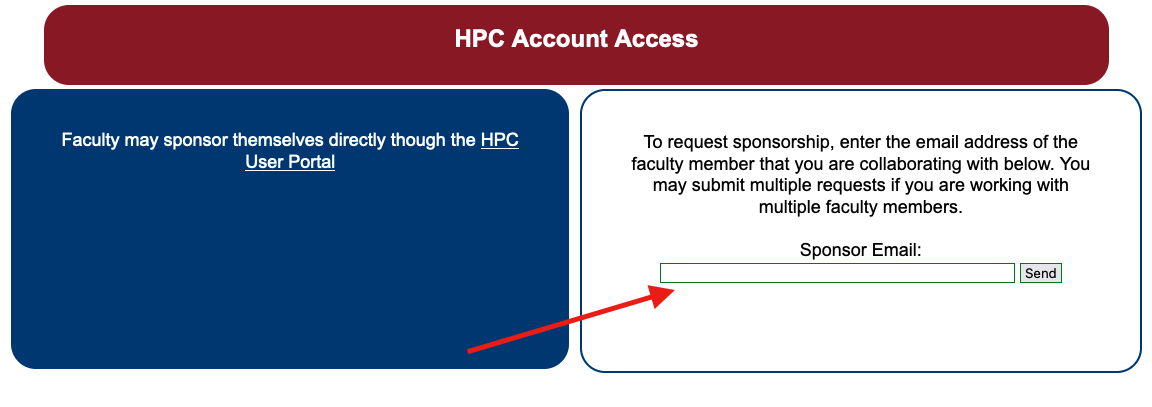
\includegraphics[width=\linewidth]{portal-sponsorship.png}\\
{\tiny\color{DarkGray} The sponsorship request on the HPC portal (2024)}
\end{column}
\end{columns}
\sourcecredit{Documentation for everything in this chapter: \url{https://hpcdocs.hpc.arizona.edu}.}
\end{frame}

% 5
\begin{frame}{What your group gets}
\small
\begin{tabular}{@{}L{0.20\textwidth}L{0.24\textwidth}L{0.50\textwidth}@{}}
\toprule
Storage & Size & Use it for \\
\midrule
\code{/home/...} & 50 GB per person & your code, scripts, small files \\
\code{/groups/<pi>} & 500 GB per group & shared, longer-term files: installs, examples \\
\code{/xdisk/<pi>} & up to 20 TB per group & running simulations and their output; lasts 150 days, with one 150-day extension \\
\bottomrule
\end{tabular}
\vspace{3mm}

\begin{tabular}{@{}L{0.20\textwidth}L{0.74\textwidth}@{}}
\toprule
Partition & What it means \\
\midrule
\code{standard} & uses your group's free monthly allocation (150{,}000 CPU hours on Puma, renewed on the first of each month); needs \code{--account=<pi group>} \\
\code{windfall} & uses no allocation, but jobs start later and can be stopped (\emph{preempted}) when others need the cores \\
\code{high\_priority} & only for groups that bought nodes in Puma \\
\bottomrule
\end{tabular}
\vspace{2mm}

Type \code{va} on the cluster to see your groups and how much allocation is left.
\end{frame}

% 6
\begin{frame}{A terminal on your own computer}
\begin{itemize}
  \item \textbf{macOS}: open \emph{Terminal} (Spotlight, then type ``terminal'').
  \item \textbf{Linux}: open a terminal window.
  \item \textbf{Windows}: \emph{PowerShell} and \emph{Windows Terminal} include the \code{ssh} command. MobaXterm and PuTTY are graphical alternatives. Ubuntu under WSL2 (chapter 2) gives you a full Linux terminal.
\end{itemize}
\vspace{2mm}
\begin{block}{A good text editor}
\small Edit code and input files with an editor that saves plain text, never a word processor. Notepad++ and Sublime Text work well on Windows; VS Code works everywhere. On Windows, set the editor to save with Unix (LF) line endings (chapter 3 shows the error you get otherwise).
\end{block}
\begin{block}{Also install}
\small VisIt for looking at results (Part V), FileZilla for moving files (this chapter), and MATLAB or Python for IB2d (Part II).
\end{block}
\end{frame}

% 7
\begin{frame}[fragile]{Logging in}
\begin{lstlisting}[style=shell]
ssh netid@hpc.arizona.edu
\end{lstlisting}
Enter your NetID password, then approve the Duo request. You arrive on the bastion host:
\begin{lstlisting}
Success. Logging you in...
This is a bastion host used to access the rest of the RT/HPC environment.

Type "shell" to access the job submission hosts for all environments
-----------------------------------------
[netid@gatekeeper ~]$ shell
\end{lstlisting}
\begin{itemize}\small
  \item Typing \code{shell} takes you to a login node. Puma is the default cluster for job submission.
  \item No VPN is needed for SSH or for Open OnDemand from off campus, because Duo protects both. The HPC VPN (\code{vpn.hpc.arizona.edu}) is needed only to open graphical windows from the cluster (X11).
  \item Older notes say to type \code{puma}, \code{ocelote} or \code{elgato} here. Those were shortcuts for choosing a cluster and are no longer needed.
\end{itemize}
\end{frame}

% 8
\begin{frame}{Open OnDemand: the cluster in a web browser}
\begin{columns}[T,onlytextwidth]
\begin{column}{0.44\textwidth}
\begin{itemize}\small
  \item Go to \url{https://ood.hpc.arizona.edu} and log in with your NetID and Duo.
  \item \textbf{Files} $\to$ \textbf{Home Directory}: browse, upload and download by drag and drop.
  \item \textbf{Clusters} $\to$ \textbf{Shell}: a terminal on a login node.
  \item \textbf{Interactive Apps}: a Linux desktop, Jupyter, MATLAB and other programs, running on compute nodes.
  \item Interactive apps ask for a group and partition: standard uses your allocation.
\end{itemize}
\end{column}
\begin{column}{0.53\textwidth}
\centering
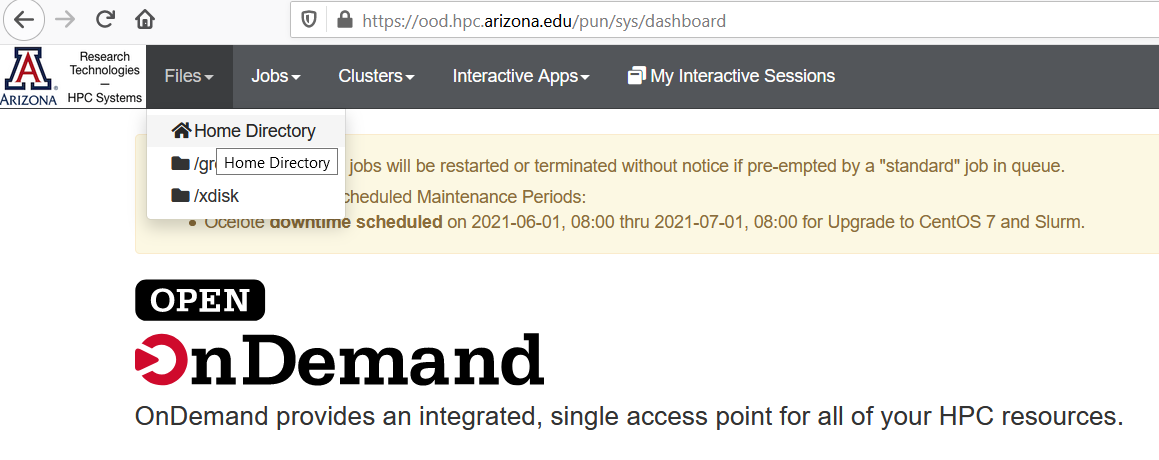
\includegraphics[width=\linewidth]{ondemand-files-menu.png}\\[2mm]
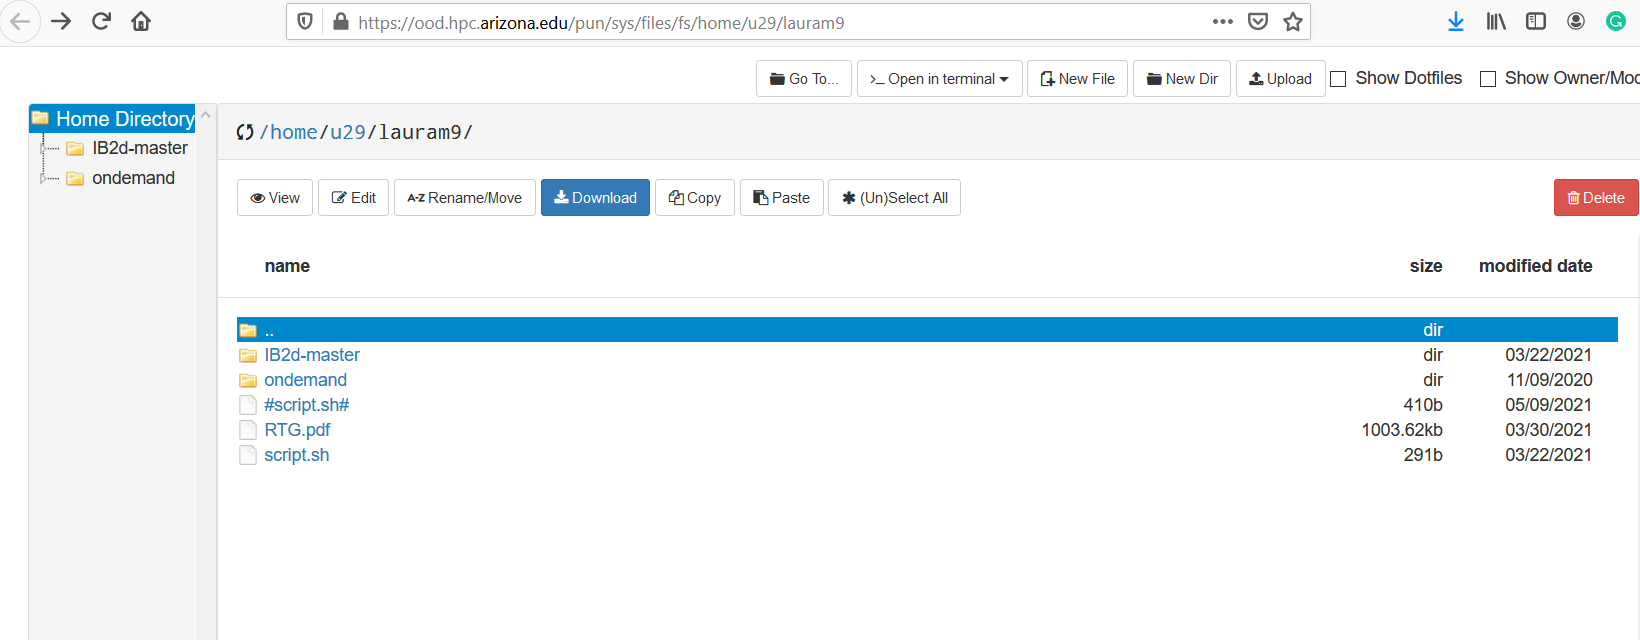
\includegraphics[width=\linewidth]{ondemand-file-browser.png}\\
{\tiny\color{DarkGray} Open OnDemand's Files menu and file browser (2022; the layout has since been updated)}
\end{column}
\end{columns}
\end{frame}

% 9
\begin{frame}{Moving files with FileZilla}
\begin{columns}[T,onlytextwidth]
\begin{column}{0.46\textwidth}
\begin{enumerate}\scriptsize
  \item Install FileZilla from \url{https://filezilla-project.org} (the client, not the server).
  \item \textbf{File $\to$ Site Manager $\to$ New Site}. On the \textbf{General} tab: Protocol \textbf{SFTP}, Host \code{filexfer.hpc.arizona.edu}, Logon Type \textbf{Interactive}, User your NetID.
  \item On the \textbf{Transfer Settings} tab, tick \emph{Limit number of simultaneous connections} and set it to \textbf{1}. Otherwise every connection asks for Duo again.
  \item \textbf{Connect}. In the first password box enter your NetID password; in the second, type \code{1} for a Duo push or enter a Duo passcode.
  \item Drag files between your computer (left) and the cluster (right).
\end{enumerate}
\end{column}
\begin{column}{0.51\textwidth}
\centering
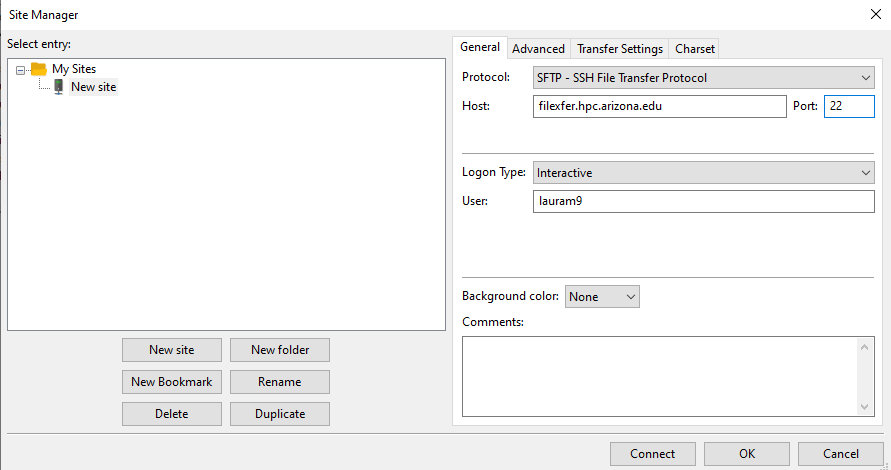
\includegraphics[width=\linewidth]{filezilla-site-manager.png}\\[2mm]
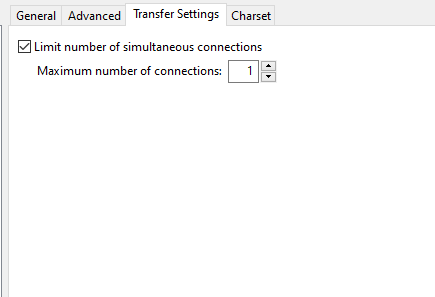
\includegraphics[width=0.55\linewidth]{filezilla-transfer-settings.png}
\end{column}
\end{columns}
\end{frame}

% 10
\begin{frame}[fragile]{Moving files from a terminal}
\textbf{sftp}: an interactive session, like a small file manager:
\begin{lstlisting}[style=shell]
sftp netid@filexfer.hpc.arizona.edu
sftp> put -r my_example          # upload a folder
sftp> get -r my_example/viz_IB2d # download a folder
sftp> exit
\end{lstlisting}
\textbf{scp} and \textbf{rsync}: one command, run on your own computer:
\begin{lstlisting}[style=shell]
scp -r my_example netid@filexfer.hpc.arizona.edu:/xdisk/<pi>/<netid>/
rsync -av netid@filexfer.hpc.arizona.edu:/xdisk/<pi>/<netid>/my_example/viz_IB2d .
\end{lstlisting}
\textbf{Many files at once}: pack them first, then send one file.
\begin{lstlisting}[style=shell]
tar -czf my_example.tar.gz my_example      # on your computer
scp my_example.tar.gz netid@filexfer.hpc.arizona.edu:/xdisk/<pi>/<netid>/
tar -xzf my_example.tar.gz                 # on the cluster, in that folder
\end{lstlisting}
\small \code{rsync} copies only what changed and can resume an interrupted copy.
\end{frame}

% 11
\begin{frame}[fragile]{Getting code with git}
For code that lives on GitHub, clone it on the cluster instead of uploading it:
\begin{lstlisting}[style=shell]
git clone https://github.com/nickabattista/IB2d.git      # first time
cd IB2d
git pull                                                  # later: get the newest version
\end{lstlisting}
\centering
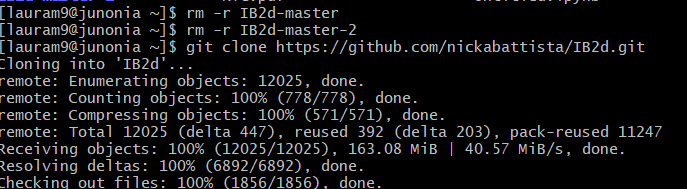
\includegraphics[width=0.75\linewidth]{git-clone-ib2d.png}\\
{\tiny\color{DarkGray} Cloning IB2d on the cluster (2022)}
\vspace{2mm}
\begin{itemize}\small
  \item The tutorials and examples are on GitHub too: \url{https://github.com/fairyflies9/Using-IB-Software}.
  \item Keep your own simulations \emph{outside} the cloned folder, so that \code{git pull} never collides with your changes.
\end{itemize}
\end{frame}

% 12
\begin{frame}{Where to keep what}
\begin{columns}[T,onlytextwidth]
\begin{column}{0.52\textwidth}
\begin{itemize}\small
  \item \textbf{Home} (\code{\textasciitilde}, 50 GB): your scripts, small codes, a personal IBAMR install if you have one.
  \item \textbf{Group folder} (\code{/groups/<pi>}, 500 GB, shared): a group IBAMR install that everyone uses, shared examples.
  \item \textbf{xdisk} (\code{/xdisk/<pi>/<netid>}): run simulations here. Output from IB simulations is large.
  \item xdisk is temporary: it lasts 150 days, plus one 150-day extension, and then it is deleted. Copy results off in time.
\end{itemize}
\end{column}
\begin{column}{0.45\textwidth}
\begin{block}{After every run}
\begin{enumerate}\small
  \item Copy the results to your computer or an external drive within a week or so.
  \item Check the copy.
  \item Delete them from the cluster:\\ \code{rm -r my\_simulation}
\end{enumerate}
\end{block}
\small A 2D run is tens of megabytes; 3D runs can reach many gigabytes. Keep results on an external drive rather than your laptop's disk.
\end{column}
\end{columns}
\end{frame}

% 13
\begin{frame}[fragile]{The shell: finding your way around}
\begin{columns}[T,onlytextwidth]
\begin{column}{0.52\textwidth}
\begin{lstlisting}[style=shell]
pwd                 # which folder am I in?
ls                  # list files
ls -lh              # with sizes and dates
ls -a               # include hidden files
cd my_example       # go into a folder
cd ..               # up one level
cd ~                # back to your home folder
mkdir runs          # make a folder
mkdir -p a/b/c      # make nested folders
cp input2d input2d.bak     # copy a file
cp -r ex1 ex1_copy         # copy a folder
mv old_name new_name       # move or rename
rm file                    # delete a file
rm -r folder               # delete a folder
\end{lstlisting}
\end{column}
\begin{column}{0.45\textwidth}
\begin{itemize}\small
  \item \alr{\code{rm} has no undo} and no trash can. Check with \code{ls} before you delete.
  \item Press \textbf{Tab} to complete file names, and the \textbf{up arrow} to recall earlier commands.
  \item \code{man ls} shows the manual for any command; \code{q} quits it.
  \item A path starting with \code{/} is absolute; anything else is relative to where you are.
\end{itemize}
\end{column}
\end{columns}
\sourcecredit{Adapted from the course guide ``Running IBAMR/IBFE on super computers'' (Nick Battista, 2014; UA version 2024).}
\end{frame}

% 14
\begin{frame}[fragile]{Looking inside files}
\begin{lstlisting}[style=shell]
cat input2d                  # print a whole file
less IB2d.log                # page through it: space, b, /search, G = end, q = quit
head -n 20 input2d           # the first 20 lines
tail -n 20 IB2d.log          # the last 20 lines
tail -f IB2d.log             # keep showing new lines as a job writes them (Ctrl-C to stop)
grep "CFL number" IB2d.log   # only the lines that contain this text
grep -c "At end" run.log     # how many lines contain it
wc -l rubber_band_512.vertex # how many lines in a file
du -sh viz_IB2d              # how much disk a folder uses
\end{lstlisting}
\begin{punchbox}
\small These are the commands you will use most when a simulation is running: \code{tail -f} to watch it, \code{grep} to pull out the numbers you care about, and \code{du} to keep an eye on disk use.
\end{punchbox}
\end{frame}

% 15
\begin{frame}[fragile]{Editing files with nano}
\begin{columns}[T,onlytextwidth]
\begin{column}{0.44\textwidth}
\begin{lstlisting}[style=shell]
nano input2d
\end{lstlisting}
\begin{itemize}\small
  \item Type to edit; move with the arrow keys.
  \item The bottom two lines list the commands; \verb|^| means the Ctrl key.
\end{itemize}
\end{column}
\begin{column}{0.53\textwidth}
\footnotesize
\begin{tabular}{@{}ll@{}}
\toprule
Keys & What they do \\
\midrule
Ctrl-O, Enter & save \\
Ctrl-X & quit (asks to save changes) \\
Ctrl-V / Ctrl-Y & next / previous page \\
Ctrl-W & search \\
Ctrl-W, then Ctrl-V & jump to the end \\
Ctrl-W, then Ctrl-Y & jump to the start \\
Ctrl-K / Ctrl-U & cut / paste a line \\
\bottomrule
\end{tabular}
\end{column}
\end{columns}
\vspace{3mm}
\small When you quit after changing a file, nano asks \emph{Save modified buffer?} Type \code{y} to save or \code{n} to throw the changes away. Opening a log file only to read it? Answer \code{n}, or use \code{less} instead.
\sourcecredit{Adapted from the course guide ``Running IBAMR/IBFE on super computers'' (Nick Battista, 2014; UA version 2024).}
\end{frame}

% 16
\begin{frame}[fragile]{Editing files with vi}
\begin{columns}[T,onlytextwidth]
\begin{column}{0.46\textwidth}
vi is on every Linux system. It has two modes:
\begin{itemize}\small
  \item \textbf{Normal mode}, where you start: keys are commands.
  \item \textbf{Insert mode}: keys type text. Press \code{i} to enter it and \textbf{Esc} to leave it.
\end{itemize}
\vspace{2mm}
\small Older course notes said to press Esc to start typing. That is backwards: \code{i} starts typing, Esc stops.
\end{column}
\begin{column}{0.52\textwidth}
\small
\begin{tabular}{@{}ll@{}}
\toprule
Keys (normal mode) & What they do \\
\midrule
\code{i} & start inserting text \\
\code{Esc} & back to normal mode \\
\code{:w} & save \\
\code{:wq} & save and quit \\
\code{:q} & quit (if nothing changed) \\
\code{:q!} & quit without saving \\
\code{:1215} & go to line 1215 \\
\code{G} / \code{gg} & go to the end / the start \\
\code{/text} & search forward for \emph{text} \\
\code{dd} / \code{u} & delete a line / undo \\
\bottomrule
\end{tabular}
\end{column}
\end{columns}
\end{frame}

% 17
\begin{frame}[fragile]{Shell scripts: commands saved in a file}
\begin{columns}[T,onlytextwidth]
\begin{column}{0.48\textwidth}
\code{hello.sh}:
\begin{lstlisting}[style=shell]
#!/bin/bash
# The first line says which program runs the file.
echo "Hello from $(hostname)"
echo "I am in $PWD"
\end{lstlisting}
Run it:
\begin{lstlisting}[style=shell]
bash hello.sh
# or make it executable once, then:
chmod +x hello.sh
./hello.sh
\end{lstlisting}
\end{column}
\begin{column}{0.49\textwidth}
\begin{itemize}\small
  \item A script runs its commands one after another, exactly as if you typed them.
  \item \code{\#} starts a comment, except in the first line, \code{\#!/bin/bash}, which names the shell.
  \item Slurm job scripts (later in this chapter) are shell scripts with extra \code{\#SBATCH} comment lines that Slurm reads.
  \item \code{bash}, the ``Bourne-again shell'', is the standard shell on Linux and on Puma; older shells such as \code{sh} and \code{csh} differ in small ways.
\end{itemize}
\end{column}
\end{columns}
\end{frame}

% 18
\begin{frame}[fragile]{Variables and quoting}
\begin{lstlisting}[style=shell]
MU=10                      # no spaces around =
echo $MU                   # => 10
echo "MU is $MU"           # => MU is 10   (double quotes expand variables)
echo 'MU is $MU'           # => MU is $MU  (single quotes do not)
RUN=run_${MU}              # braces mark where the name ends => run_10
NSTEPS=$(grep -c "At end" run.log)    # $( ) captures a command's output
echo "finished $NSTEPS steps"
\end{lstlisting}
\begin{itemize}\small
  \item \code{MU = 10}, with spaces, is an error: the shell tries to run a command called \code{MU}.
  \item Put double quotes around variables that hold file names, so names with spaces survive: \code{cp "\$FILE" backup/}.
  \item \code{\$HOME}, \code{\$USER} and \code{\$PWD} are always set; Slurm adds variables such as \code{\$SLURM\_NTASKS} inside jobs.
\end{itemize}
\sourcecredit{Shell examples in this chapter rewritten from the 2018 course deck ``Running many simulations, part 1'', which drew on Learn X in Y minutes (bash), the Rutgers Bash Beginners Guide, and DigitalOcean's awk tutorial.}
\end{frame}

% 19
\begin{frame}[fragile]{Loops and tests}
\begin{columns}[T,onlytextwidth]
\begin{column}{0.50\textwidth}
\begin{lstlisting}[style=shell]
# make three run folders
for MU in 100 10 1; do
    mkdir -p run_MU$MU
    echo "made run_MU$MU"
done

# numbers 1 to 5
for i in {1..5}; do echo $i; done
for ((i=1; i<=5; i++)); do echo $i; done
\end{lstlisting}
\end{column}
\begin{column}{0.47\textwidth}
\begin{lstlisting}[style=shell]
if [ -f input2d ]; then
    echo "input2d is here"
else
    echo "no input2d"
fi

# run the second command only if the first worked
cmake --build build && echo "build OK"
# ... only if it failed
cmake --build build || echo "build FAILED"
\end{lstlisting}
\end{column}
\end{columns}
\begin{itemize}\small
  \item Inside \code{[ ]} the spaces are required: \code{[ -f input2d ]}.
  \item Useful tests: \code{-f} a file exists, \code{-d} a folder exists, \code{"\$a" == "\$b"} equal strings, \code{\$x -lt 5} a number less than 5.
\end{itemize}
\end{frame}

% 20
\begin{frame}[fragile]{Redirection and pipes}
\begin{lstlisting}[style=shell]
mpirun -np 4 ./build/main2d input2d > run.log          # screen output into a file
mpirun -np 4 ./build/main2d input2d > run.log 2>&1     # ... errors too
echo "MU = 10" >> notes.txt                            # append instead of overwrite
grep "integral{F}" run.log | tail -1                    # the last force line
grep "CFL number" IB2d.log | awk '{print $NF}' > cfl.txt   # just the numbers
\end{lstlisting}
\begin{itemize}\small
  \item Every program has three streams: \textbf{input} (0), \textbf{output} (1) and \textbf{errors} (2). \code{>} sends output to a file, \code{2>\&1} sends errors to the same place.
  \item \code{|} (a \emph{pipe}) sends one command's output into the next command as its input. Chains of small commands do a lot of everyday data handling.
  \item \code{> file} overwrites \code{file} without asking.
\end{itemize}
\end{frame}

% 21
\begin{frame}[fragile]{Three tools for text: grep, sed, awk}
\begin{lstlisting}[style=shell]
grep -n "MU" input2d                     # lines containing MU, with line numbers
grep -r "viz_dump_interval" .            # search every file below this folder
sed -n '10,20p' input2d                  # print lines 10 to 20
sed -i 's/^END_TIME .*/END_TIME = 0.5/' input2d    # replace the END_TIME line (edits the file!)
awk '{print $1, $2}' F.00400             # print columns 1 and 2
awk '/^MU[ \t]*=/ {print "MU = 10"; next} {print}' input2d > input2d.new   # replace by name
awk -F, '{s += $3} END {print s/NR}' data.csv      # average of column 3 in a CSV file
\end{lstlisting}
\begin{itemize}\small
  \item \code{grep} finds lines, \code{sed} edits lines, \code{awk} works with columns and does arithmetic.
  \item \code{sed -i} changes the file in place: make a copy first (\code{cp input2d input2d.bak}).
  \item awk splits each line into fields \code{\$1}, \code{\$2}, \ldots{} at spaces; \code{-F,} splits at commas. \code{\$NF} is the last field, \code{NR} the line number. A \code{BEGIN} or \code{END} block runs before or after all lines.
\end{itemize}
\end{frame}

% 22
\begin{frame}[fragile]{Software on Puma: modules}
Software is installed as \textbf{modules}, which you load on a compute node:
\begin{lstlisting}[style=shell]
interactive                 # a compute node: 1 core, 1 hour, windfall
module avail                # everything that is installed
module avail matlab         # just MATLAB versions
module load gnu13 openmpi5  # the compilers and MPI used for IBAMR in this course
module list                 # what is loaded now
module unload openmpi5      # remove one
\end{lstlisting}
What \code{interactive} does (Puma, 2024):
\begin{lstlisting}[style=tiny]
Run "interactive -h for help customizing interactive use"
Submitting with /usr/local/bin/salloc --job-name=interactive --mem-per-cpu=4GB --nodes=1 --ntasks=1 --time=01:00:00 --account=windfall --partition=windfall
NOTICE: Submitting to the windfall queue may result in longer wait times or preemption. Consider submitting with an account (-a your_group).
salloc: Granted job allocation 10095845
\end{lstlisting}
\small \code{interactive -a <your group>} uses your group's allocation and usually starts sooner; \code{interactive -h} lists the options for more cores or time.
\end{frame}

% 23
\begin{frame}[fragile]{A Slurm batch script}
\begin{columns}[T,onlytextwidth]
\begin{column}{0.55\textwidth}
\begin{lstlisting}[style=slurm,basicstyle=\ttfamily\tiny\color{BlackGray}]
#!/bin/bash
### Part 1: what to reserve
#SBATCH --job-name=hello_world
#SBATCH --output=%x-%j.out        # %x = job name, %j = job number
#SBATCH --account=<PI GROUP>      # required
#SBATCH --partition=standard      # or windfall
#SBATCH --nodes=1
#SBATCH --ntasks=1                # cores (MPI processes)
#SBATCH --mem-per-cpu=4gb
#SBATCH --time=00:10:00           # hh:mm:ss
### #SBATCH --mail-type=ALL       # optional: email at start and end
### #SBATCH --mail-user=<netid>@arizona.edu

### Part 2: what to run
module load gnu13
cd "$SLURM_SUBMIT_DIR"
./hello_world
\end{lstlisting}
\end{column}
\begin{column}{0.42\textwidth}
\begin{itemize}\scriptsize
  \item Lines starting \code{\#SBATCH} are read by Slurm. To switch one off, add more \code{\#}: \code{\#\#\# \#SBATCH \ldots}
  \item \textbf{Part 1} reserves resources: cores, memory, time, group, partition.
  \item \textbf{Part 2} is an ordinary shell script that runs on the compute node.
  \item Ask for a little more time than you need. A job that runs out of time is stopped.
  \item Every example in this tutorial has a ready \code{job.slurm} (chapter 3).
\end{itemize}
\end{column}
\end{columns}
\sourcecredit{Based on the UArizona HPC quick-start template, as used in the course decks (2022); updated module and memory lines.}
\end{frame}

% 24
\begin{frame}[fragile]{Submitting, watching and checking jobs}
\begin{lstlisting}[style=shell]
sbatch job.slurm                 # submit: "Submitted batch job 10095996"
squeue --me                      # your jobs: ST = PD (pending) or R (running)
scancel 10095996                 # stop a job
sacct -j 10095996 --format=JobID,State,Elapsed,AllocCPUS,MaxRSS,ExitCode   # afterwards
\end{lstlisting}
\begin{itemize}\small
  \item \code{squeue --me} is the same as \code{squeue -u <netid>}. The \code{NODELIST(REASON)} column says why a job is waiting, for example \code{(Priority)}.
  \item \code{sacct} reports what a finished job used: \code{Elapsed} time and \code{MaxRSS}, the most memory one process used. Use them to size the next request.
  \item Write down each job number with a note of what it runs; chapter 3 shows how to follow an IBAMR job.
\end{itemize}
\sourcecredit{\code{squeue --me} and \code{sacct} usage from the instructor's 2026 Puma notes for IB2d runs.}
\end{frame}

% 25
\begin{frame}[fragile]{MATLAB and Python jobs (for IB2d)}
\begin{columns}[T,onlytextwidth]
\begin{column}{0.52\textwidth}
\begin{lstlisting}[style=slurm]
#!/bin/bash
#SBATCH --job-name=ib2d_run
#SBATCH --account=<PI GROUP>
#SBATCH --partition=standard
#SBATCH --ntasks=1
#SBATCH --mem=16gb
#SBATCH --time=04:00:00

module load matlab
cd "$SLURM_SUBMIT_DIR"
matlab -nodisplay -nosplash < main2d.m
\end{lstlisting}
\end{column}
\begin{column}{0.45\textwidth}
\begin{itemize}\scriptsize
  \item IB2d runs on one core, so \code{--ntasks=1}; ask for enough memory for the grid you use.
  \item For the Python version of IB2d, load a Python module instead, for example \code{module load python/3.11/3.11.4}, and run \code{python main2d.py}. Module names change; check with \code{module avail python}.
  \item If MATLAB asks for a MathWorks sign-in, start an \code{interactive} session, load the same module, run \code{matlab} once and sign in. Do not do this on a login node.
  \item Part II covers IB2d itself.
\end{itemize}
\end{column}
\end{columns}
\sourcecredit{Adapted from the course decks ``HPC @ UA, running ib2d and IBAMR'' (2021--2022) and the instructor's 2026 Puma notes.}
\end{frame}

% 26
\begin{frame}{Other University computing services}
These are useful but not needed for this tutorial:
\begin{itemize}\small
  \item \textbf{U-System}: a general-purpose Unix account (\url{https://account.arizona.edu}), reached by SSH to \code{u.arizona.edu}.
  \item \textbf{Virtual desktops} (VCAT, \url{https://arizona.apporto.com}): Windows desktops in a browser with licensed software such as ANSYS, MATLAB, Blender and MeshLab, without installing anything. They can be slow when many people use them.
  \item \textbf{Jupyter and MATLAB in a browser}: through Open OnDemand's Interactive Apps on Puma.
\end{itemize}
\vspace{2mm}
\begin{punchbox}
\small Check what each service offers on the University's IT pages before relying on it; the lists of software change every year.
\end{punchbox}
\sourcecredit{From the course deck ``HPC and computing resources @ UA'' (2022).}
\end{frame}

% 27
\begin{frame}{What changed since the older course notes}
\small
\begin{tabular}{@{}L{0.42\textwidth}L{0.52\textwidth}@{}}
\toprule
Older notes say & Now \\
\midrule
log in to Puma, Ocelote or El Gato; type \code{puma} or \code{ocelote} & Puma only; type \code{shell} at the bastion \\
UNC clusters: Kure, KillDevil, Dogwood, Longleaf (LSF \code{bsub}, then Slurm) & see Part X, chapter X1 \\
start a VPN before logging in & not needed for SSH or Open OnDemand \\
documentation on Confluence (\code{public.confluence.arizona.edu}) & \url{https://hpcdocs.hpc.arizona.edu} \\
\code{module load gnu/5.4.0} & \code{module load gnu13 openmpi5} for IBAMR \\
xdisk is deleted after 300 days & 150 days plus one 150-day extension: 300 at most \\
\code{\#SBATCG --output} (a typo, so the line was ignored) & \code{\#SBATCH --output} \\
\code{-t 1} means one hour & \code{-t 1} means one \emph{minute}; write \code{--time=01:00:00} \\
in vi, press Esc to type & press \code{i} to type, Esc to stop \\
\bottomrule
\end{tabular}
\end{frame}

% 28
\begin{frame}{Summary}
\begin{enumerate}\small
  \item Get an account on the HPC portal and join your PI's group; the group name goes after \code{--account}.
  \item Log in with \code{ssh netid@hpc.arizona.edu}, approve Duo, type \code{shell}. Or use Open OnDemand.
  \item Move files with FileZilla, \code{sftp}, \code{scp} or \code{rsync} through \code{filexfer.hpc.arizona.edu}; get code with \code{git clone}.
  \item Code in home or the group folder; simulations on xdisk; copy results off and delete them.
  \item Learn the shell: \code{ls}, \code{cd}, \code{less}, \code{grep}, an editor, and short scripts.
  \item Work on compute nodes only: \code{interactive} for short tests, \code{sbatch} for real runs, \code{squeue --me} and \code{sacct} to follow them.
\end{enumerate}
\vspace{2mm}
\begin{homebox}
\small Next, chapter 2 installs IBAMR, and chapter 3 builds and runs your first simulation.
\end{homebox}
\end{frame}

% 29
\begin{frame}{References and credits}
\small
\begin{itemize}
  \item UArizona HPC documentation: \url{https://hpcdocs.hpc.arizona.edu} (system access, storage, allocations, Open OnDemand, file transfer).
  \item FileZilla: \url{https://filezilla-project.org}.
  \item Course material reused here: ``Running IBAMR/IBFE on super computers'' (Nick Battista, 2014; UA version 2024); ``HPC and computing resources @ UA'' and ``HPC @ UA, running ib2d and IBAMR'' (2021--2022); ``Running many simulations, part 1'' (2018); the instructor's Puma notes (2026).
  \item Shell references the 2018 deck drew on: Learn X in Y minutes, bash (\url{https://learnxinyminutes.com/docs/bash/}); Machtelt Garrels, \emph{Bash Guide for Beginners}; DigitalOcean, ``How to use the awk language to manipulate text in Linux''.
  \item Screenshots are from the course decks (2022--2024).
\end{itemize}
\end{frame}

\end{document}
